\chapter{$^{156}$Gd Results}

$^{156}$Gd is of interest to study due to the deformed nature of the nucleus. It is known to have 6 $0^+$ states, allowing for many potential transitions between two states of the same $J^\pi$. This data was taken with ICEBall and GEORGINA. The experiment used an enriched $^{154}$Sm target of 1.7 $mg/cm^2$ thickness, as discussed in Chapter \ref{chap:setup} and shown in Table \ref{tab:target}.

\section{Ground State Band Confirmation}

Looking at the singles spectra of the data, several prominent peaks stand out, seen in Figure \ref{fig:156_Singles}. In the $\gamma$-spectrum on top, there are three prominent peaks from 100 to 400 keV. These peaks are the ground state band transitions from the $2^+$ state up to the $8^+$ state. The transition from the $2^+$ state to the ground state is only 89 keV, and while visible, suffers from a steep efficiency drop-off at that energy, and a large background due to x-rays. The strong peak just beyond 500 keV is the 511 keV annihilation peak. The conversion electron spectrum on the lower half of Figure \ref{fig:156_Singles} has clear $K$-shell and $L$-shell peaks corresponding to these ground state band transitions. 

\begin{figure}[!]
    \centering
    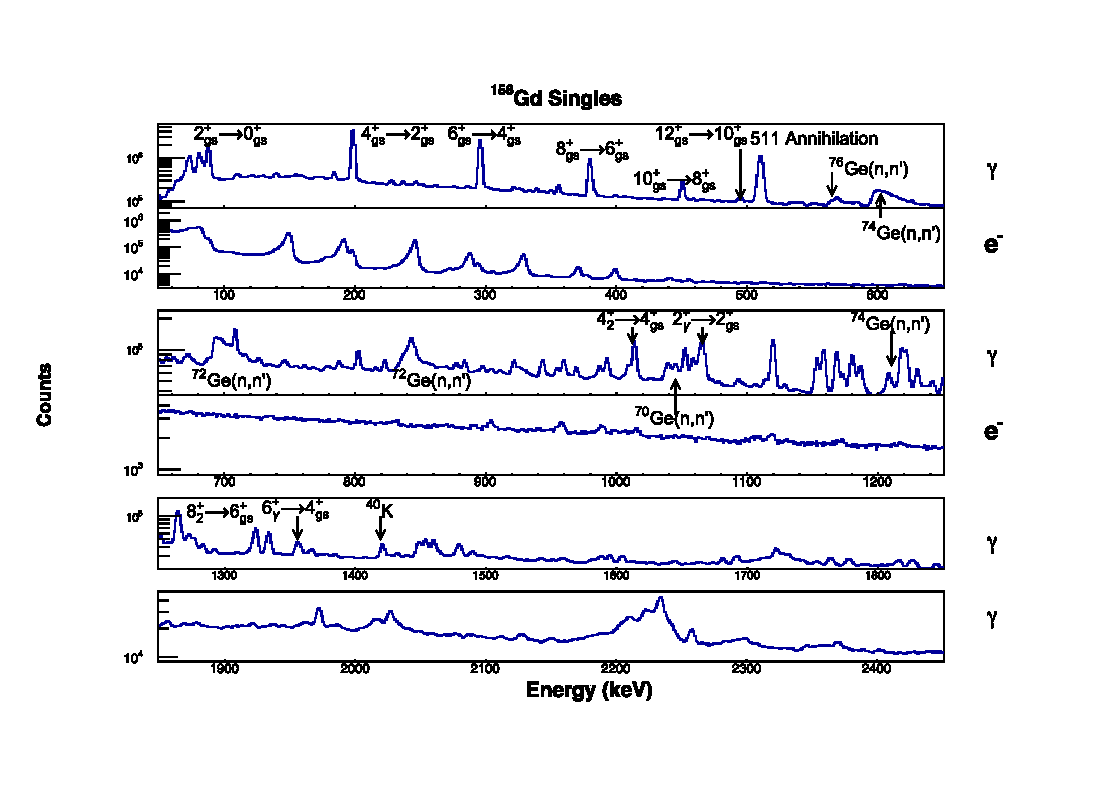
\includegraphics[scale=0.9]{156GdTablesAndFigs/156Gd_Singles_Label.eps}
    \caption{Singles spectra of $^{156}$Gd. Spectra are labeled with the particles being detected, the energies of the $\gamma$ and electron spectra aligned for identification. In the $\gamma$ spectrum, several lines of note are labeled. These are the ground-state band lines as well as other transitions of interest. Below 100 keV is a combination of x-rays and the 89 keV gamma from the ground state band. In the conversion electron spectrum, the large peaks up to approximately 350 keV are from the ground state band. These large peaks make the ground state band a good diagnostic, but also emphasize the need for coincidence gating, as the conversion electron spectrum is flooded by the ground state band electrons. The large peak at low energy is cut off due to the threshold. It is a combination of background and the 89L peak. Transitions in the higher energy regime of the $\gamma$ spectrum cannot be determined without gating, due to additional background from the experimental room.}
    \label{fig:156_Singles}
\end{figure}

As in the previous chapter, these transitions in the ground state are the first lines looked at in the data. These are all pure E2 multipole transitions, making them a diagnostic on the data compared with the theoretical coefficients from BrIcc\citep{kibedi08:_BRICC}. The transitions from $2^+$ to $10^+$ are summarized and compared with theory in Table \ref{tab:156Gd_Single_ICC_GS}.

\begin{landscape}
\footnotesize
    \begin{longtable}{c|c|c|c|c|c|c|c|c|c}
    \caption{$^{156}$Gd Ground State Band Internal Conversion Coefficients from Singles}
        \label{tab:156Gd_Single_ICC_GS}\\
    \toprule
$E$ (keV)	&	$J^{\pi}	\rightarrow	J^{\pi}$	&	$E_i$ (keV)	&	$E_f$ (keV)	&	$T_{1/2}$ (fs)	&	Multipolarity	&	Shell & $\alpha$ (This Work)	&	$\alpha$  (Th)	&	$\alpha$ (Konijn)	\\
\hline		
\endfirsthead
    \caption[]{$^{156}$Gd Ground State Band Internal Conversion Coefficients from Singles}\\
    \toprule
$E$ (keV)	&	$J^{\pi}	\rightarrow	J^{\pi}$	&	$E_i$ (keV)	&	$E_f$ (keV)	&	$T_{1/2}$ (fs)	&	Multipolarity	&	Shell & $\alpha$ (This Work)	&	$\alpha$  (Th)	&	$\alpha$ (Konijn)	\\
\hline		
\endhead
\endfoot
\multicolumn{10}{p{1.4\textwidth}}{A list of the ground state conversion coefficients from $^{156}$Gd. Multipolarities and mixing ratios were taken from NNDC. Unless otherwise stated, the $\alpha$ values are $\alpha_K$. An angular distribution correction has been applied based on multipolarities for pure transitions, and those with known mixing ratios. The first error is statistical, the second is systematic. Numbers are compared with Konijn et al. \citep{konijn81:_156gd} Starred values in the Konijn data were used as calibration points.}
\endlastfoot
198.58	&	$4^+	\rightarrow	2^+$	&	288.187	&	88.97	&	111900	&	E2	& K &	0.1667 (4)$^{+46}_{-45}$	&	0.1565 (22)	&	0.199 (36)	\\
	&				&		&		&		&		& L &	0.0537 (1)$^{+16}_{-15}$	&	0.0531 (8)	&		\\
	&			&		&		&		&		& M &	0.0170 (1) (5)	&	0.0122 (2)	&		\\ \hline
296.04	&	$6^+	\rightarrow	4^+$	&	584.715	&	288.187	&	15800	&	E2 & K	&	0.0572 (1) (18)	&	0.0477 (7)	&	0.04683*	\\
	&				&		&		&		&	& L	&	0.0121 (1) (4)	&	0.0115 (2)	&		\\
	&				&		&		&		&	& M	&	0.0036 (1) (1) &	0.0026 (1)	&		\\ \hline
379.92	&	$8^+	\rightarrow	6^+$	&	965.134	&	584.715	&	4320	&	E2 & K	&		0.0274 (1) (9)	&	0.0235 (4)	&	0.038 (10)	\\
	&				&		&		&		&	& L	&	0.0050 (1) (2)	&	0.0048 (1)	&		\\
	&				&		&		&		&	& M	&	0.0013 (1) (1)	&	0.0011 (1)	&		\\ \hline
450.64	&	$10^+	\rightarrow	8^+$	&	1416.078	&	965.134	&	1900	&	E2	& K &	0.0152 (2) (5)	&	0.01483 (21)	& 0.0145*		\\
	&				&		&		&		&	& L	&	0.0028 (1) (1)	&	0.00279 (4)	&		\\
	&				&		&		&		&	& M	&	0.0010 (1) (1)	&	0.000621 (9)	&		\\ 
\bottomrule
    \end{longtable}
\end{landscape}

Unlike the $^{154}$Gd data, there did not appear to be contaminants in these ground state lines, outside of the $2^+\rightarrow0^+$ transition. This transition was also considered unreliable, as the low energy of the $\gamma$-ray put it before the efficiency turnover. The change in efficiency in the HPGe detectors is steep in this region, leading to large uncertainty.

\section{Gates on the Ground State Band}

The transitions of the ground state band were the most prominent peaks in the spectra (Figure \ref{fig:156_Singles}). The high number of counts in these peaks made them prime candidates to gate on and build up a level scheme. Only the $\gamma$ components were gated on, as the electron components wide width made it difficult to gate on the whole of the peak without contaminants. Figures \ref{fig:156_2to0}, \ref{fig:156_4to2}, \ref{fig:156_6to4}, and \ref{fig:156_8to6} are the result of these gates. Unlike the gates in $^{154}$Gd, the $4^+\rightarrow2^+$ gate was the most fruitful, due to the challenges of the $2^+\rightarrow0^+$ transition posed. 

\afterpage{\clearpage\begin{figure}[!]
    \centering
    \begin{subfigure}{\textwidth}
    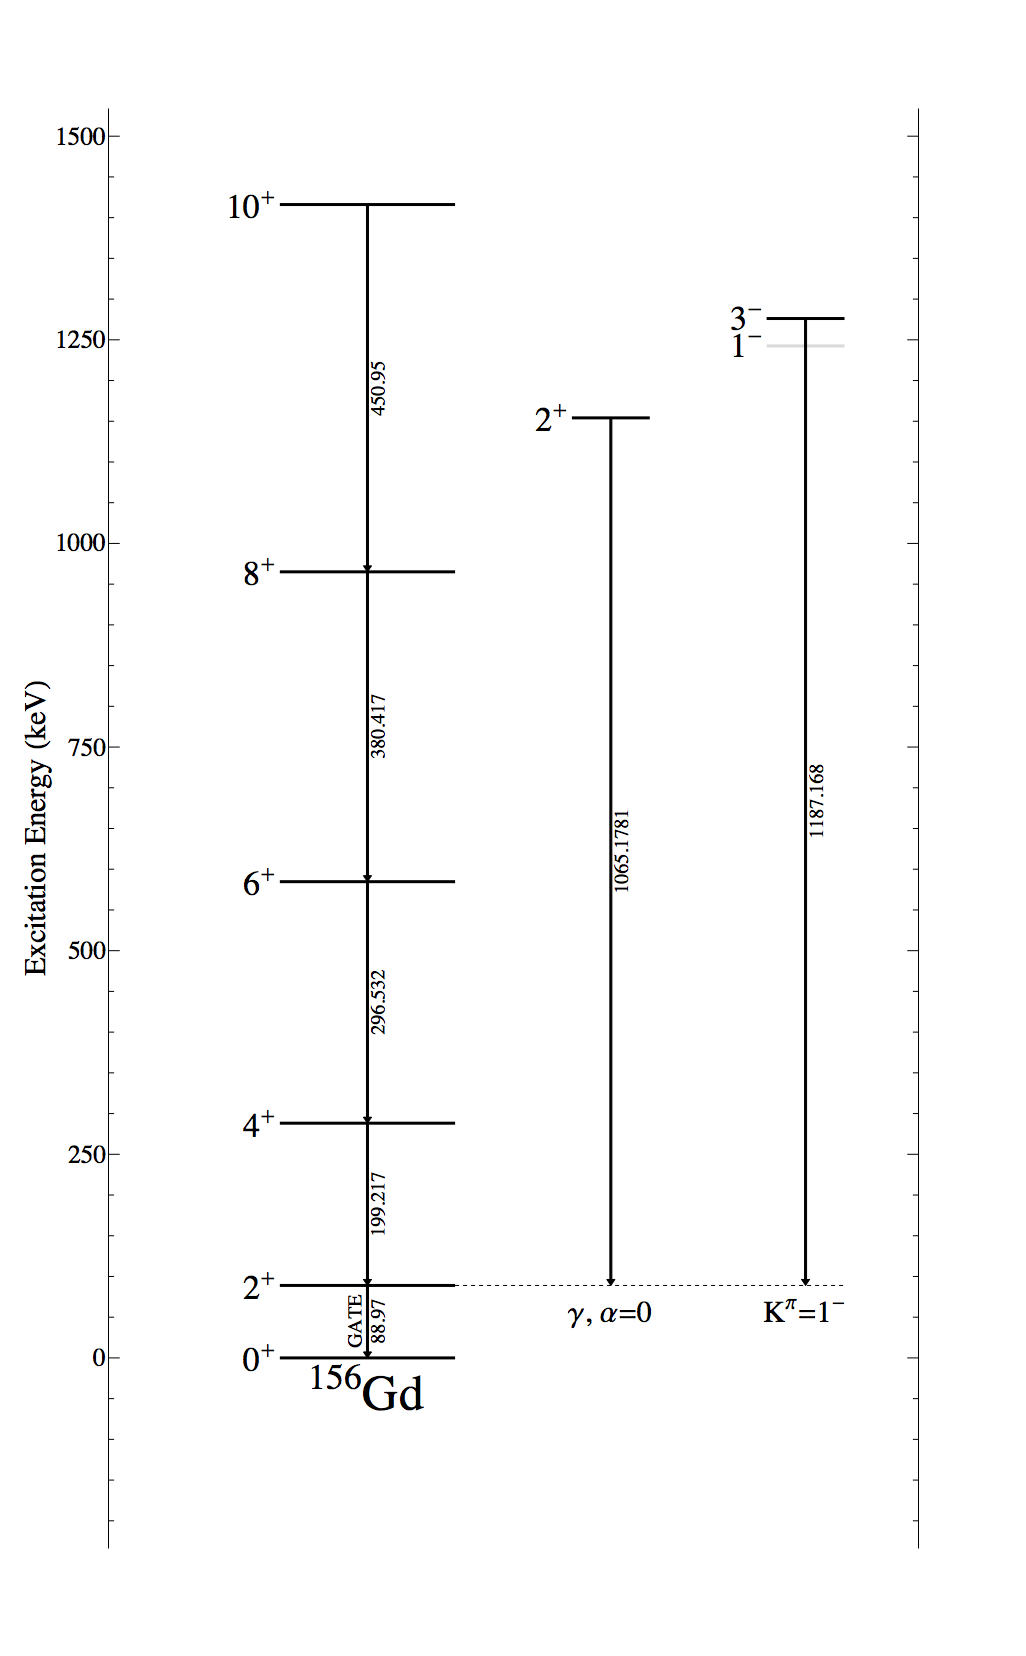
\includegraphics[scale=0.4]{156GdTablesAndFigs/156Gd_2to0.eps}
    \caption{\label{fig:156_2to0level}Level Scheme of $^{156}$Gd. The gamma ray of the $2^+$\rightarrow$0^+$ (89 keV) transition in the ground state was gated on. It was then compared with the gated spectrum from the gamma ray of the $4^+$\rightarrow$2^+$ (199 keV) transition in the ground state. Peaks only appearing in the first gate were assumed to go into the $2^+$ state, and assignments were made. Due to the low energy of the $2^+$\rightarrow$0^+$ transition, the efficiency was lower, and it is likely that transitions into the $2^+$ state were missed. The levels are organized by band. The lower levels of the band, unseen by gamma rays in this gate, are in gray.}
    \end{subfigure}
    \captionlistentry{Level scheme and spectrum of $^{156}$Gd based on the $2^+\rightarrow0^+$ transition.}
    \label{fig:156_2to0}
    \end{figure}
\begin{landscape}
    \begin{figure}
    \ContinuedFloat
    \begin{subfigure}{1.4\textwidth}
    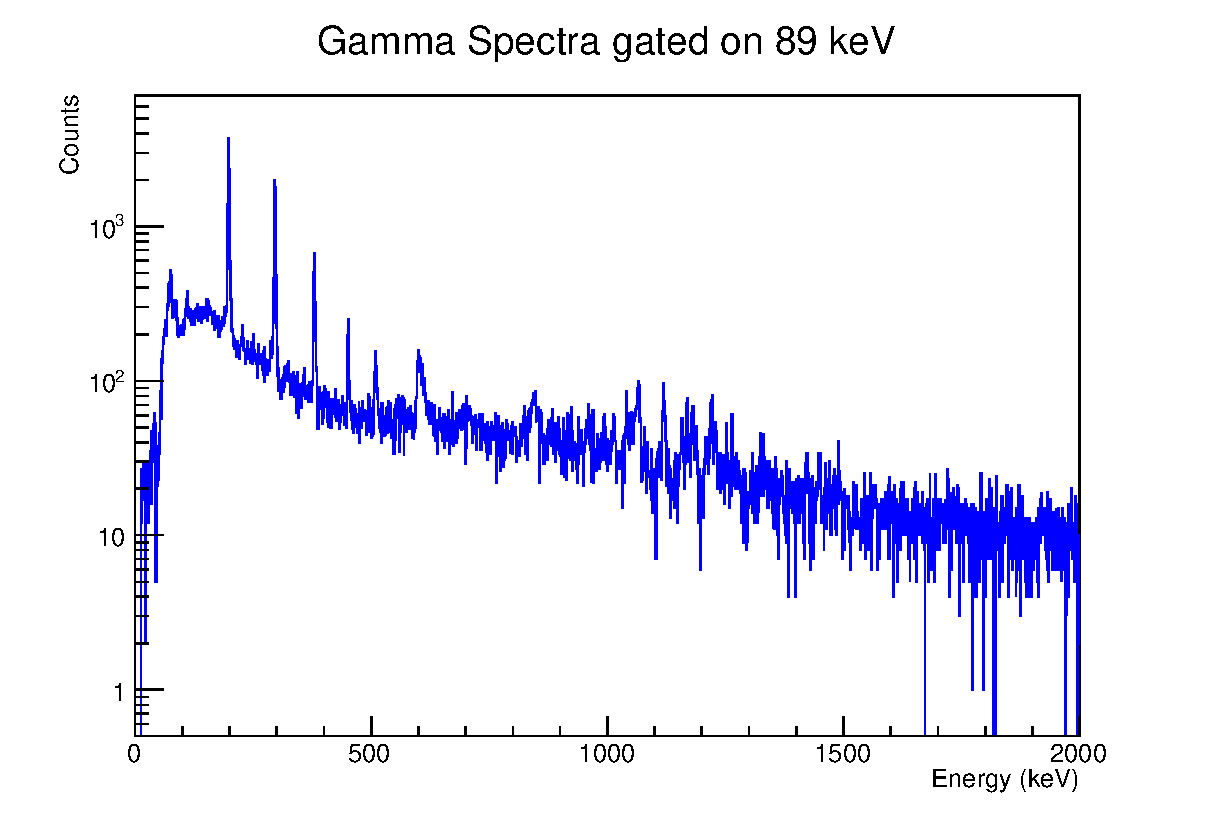
\includegraphics[]{156GdTablesAndFigs/89GateSpectrum.eps}
    \caption{Gamma spectrum gated on 89 keV, corresponding to the $2^+\rightarrow0^+$ transition.}
    \label{fig:156_2to0spec}
    \end{subfigure}
\end{figure}
\end{landscape}}

\afterpage{\clearpage\begin{landscape}
\begin{figure}
    \centering
    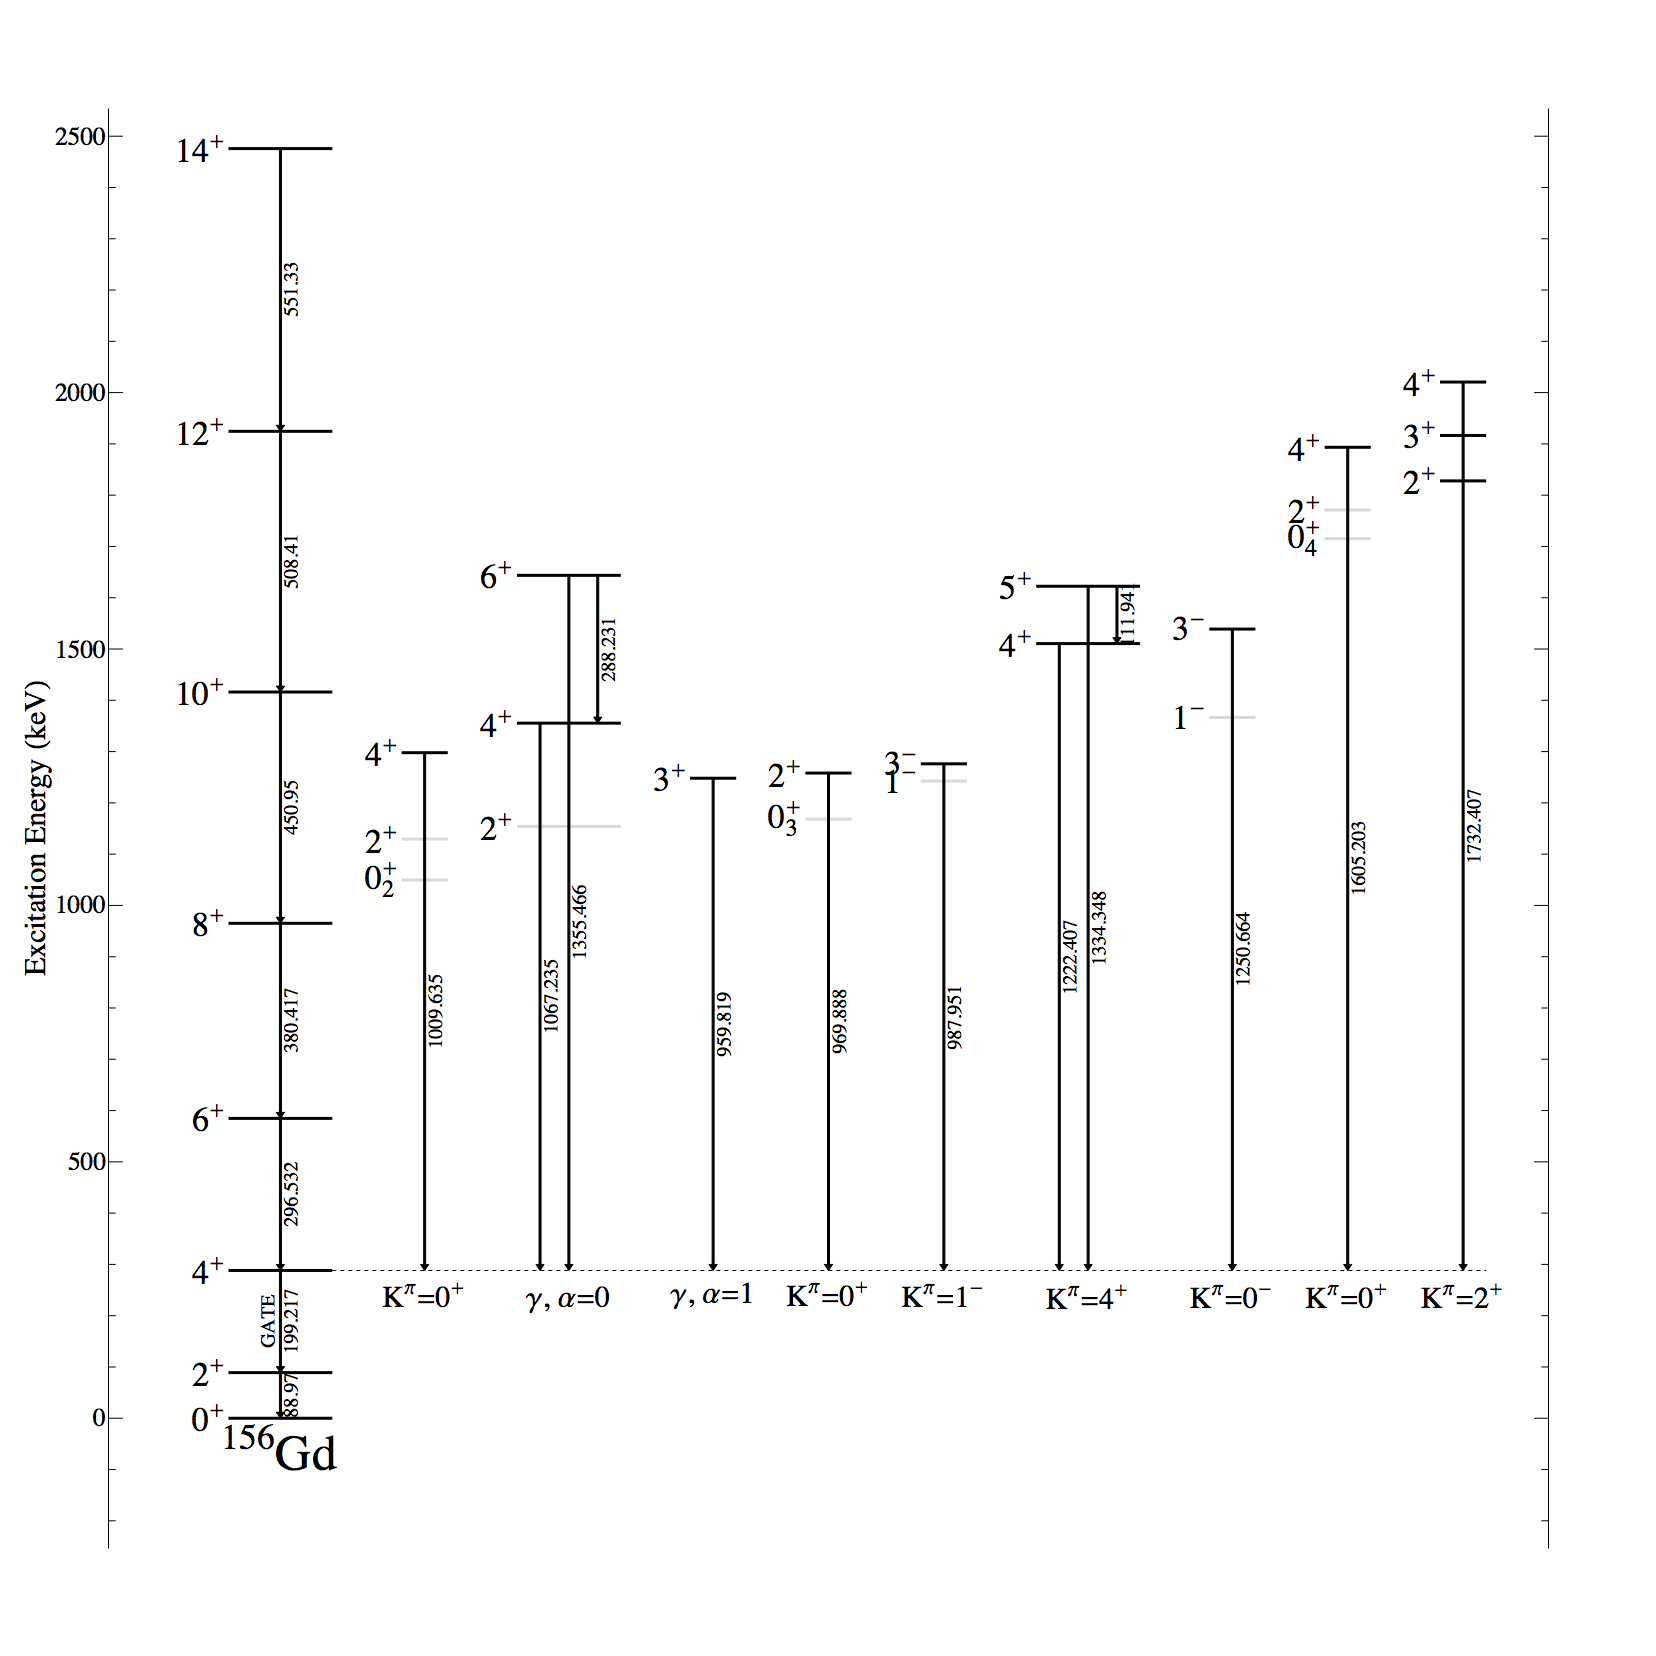
\includegraphics[scale=0.4]{156GdTablesAndFigs/156Gd_4to2.eps}
    \caption{Level Scheme of $^{156}$Gd. The gamma ray of the $4^+$\rightarrow$2^+$ (199 keV) transition in the ground state was gated on. It was then compared with the gated spectrum from the gamma ray of the $6^+$\rightarrow$4^+$ (296 keV) transition in the ground state. Peaks only appearing in the first gate were assumed to go into the $4^+$ state, and assignments were made. Additionally, these peaks were also gated on, to look for cascades leading into the $4^+$ state, which were found in several cases. The levels are organized by band. The lower levels of the band, unseen by gamma rays in this gate, are in gray.}
    \label{fig:156_4to2}
\end{figure}
\end{landscape}}

\afterpage{\clearpage\begin{figure}
    \centering
    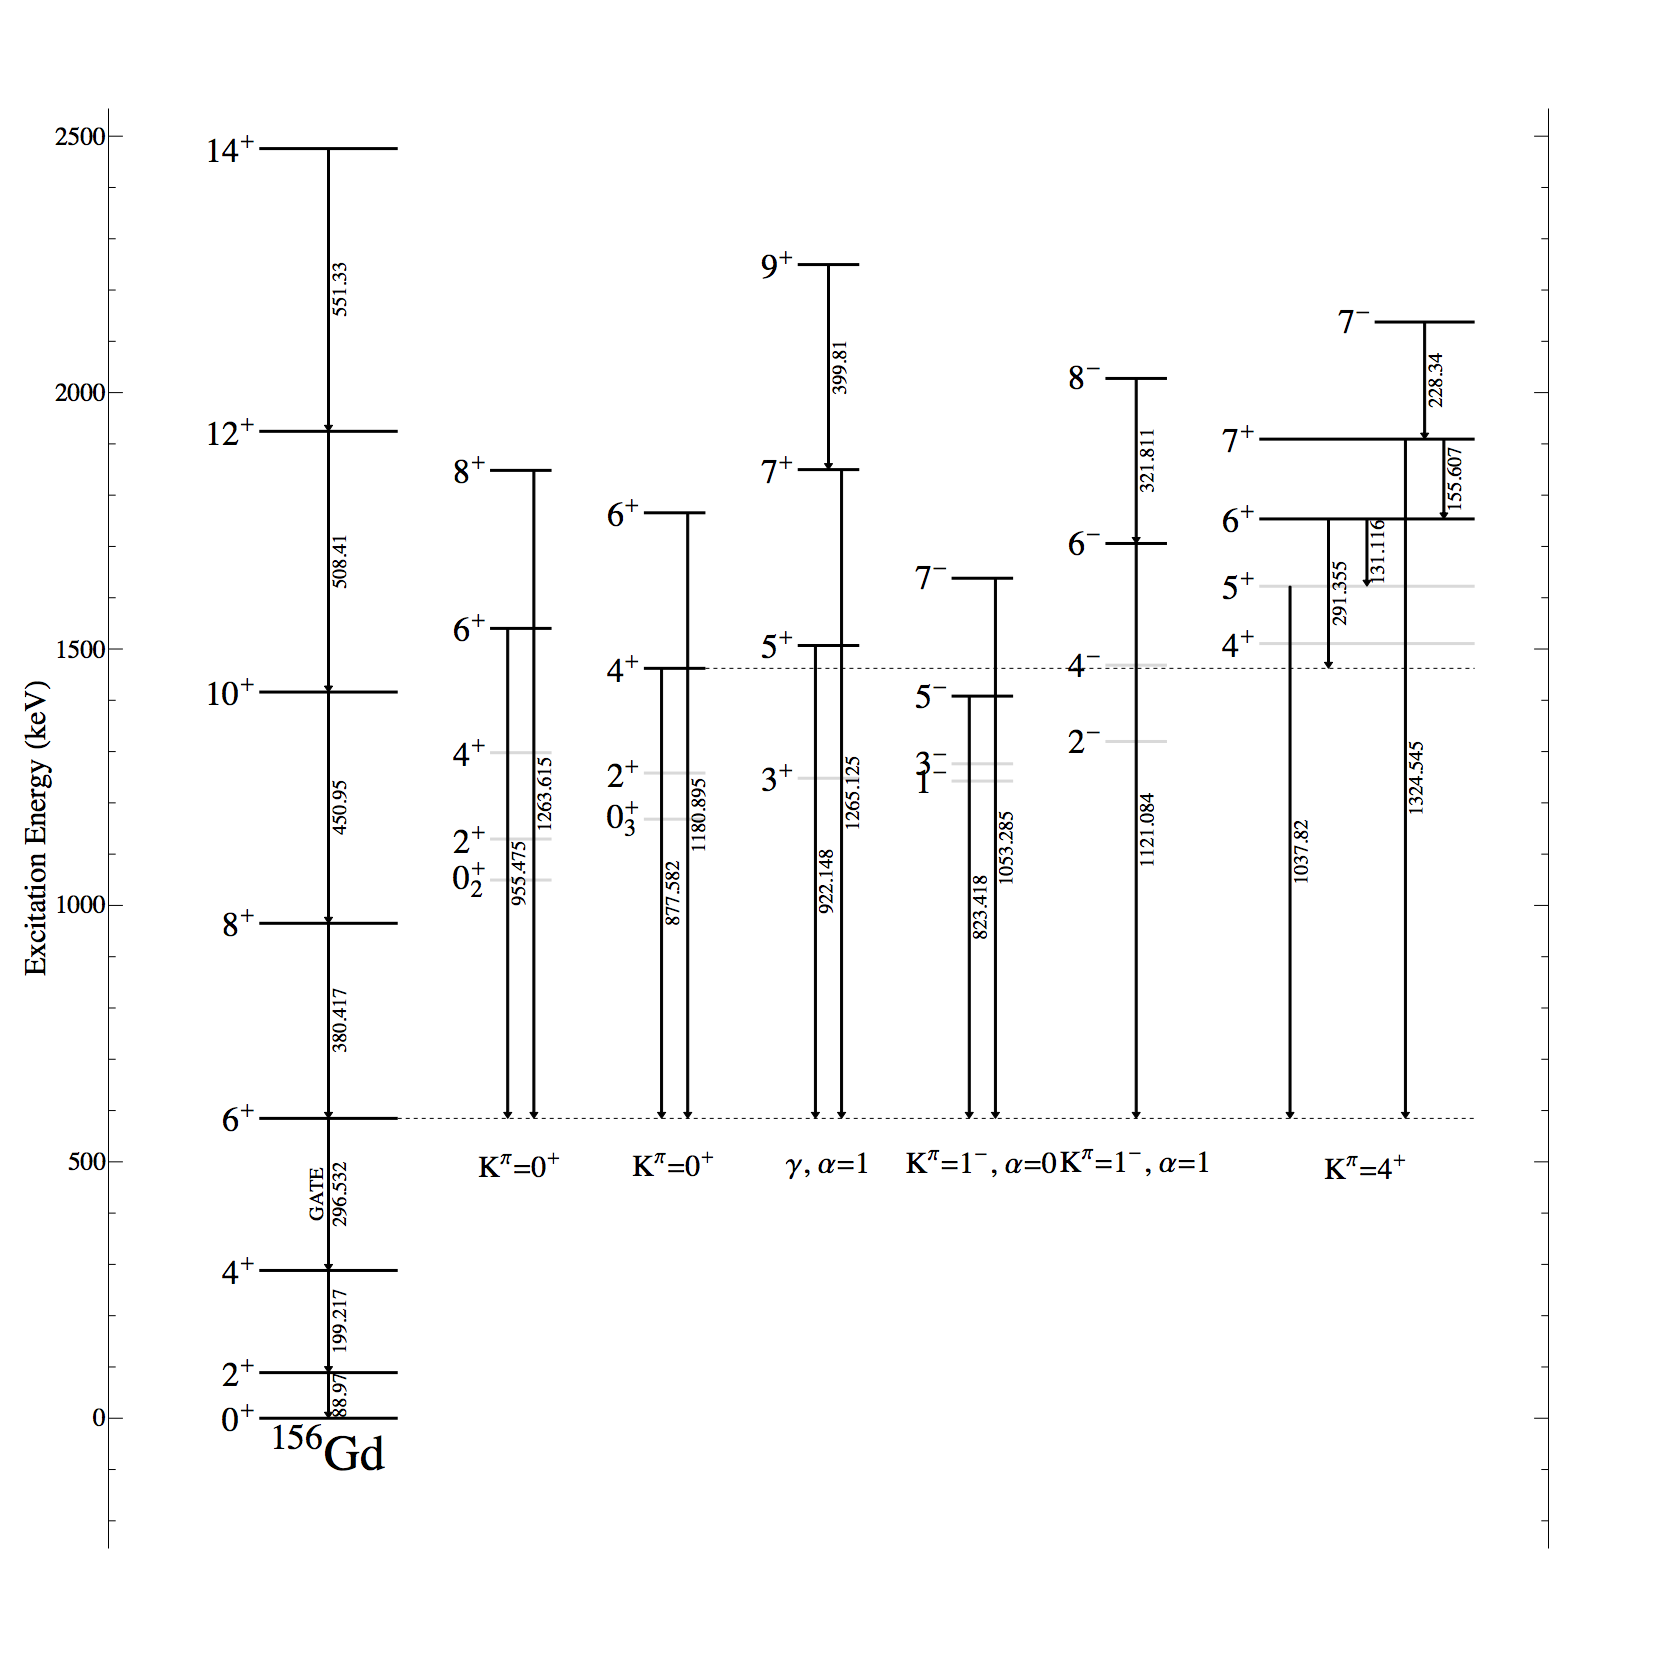
\includegraphics[scale=0.28]{156GdTablesAndFigs/156Gd_6to4.png}
    \caption{Level Scheme of $^{156}$Gd. The gamma ray of the $6^+$\rightarrow$4^+$ (296 keV) transition in the ground state was gated on. It was then compared with the gated spectrum from the gamma ray of the $8^+$\rightarrow$6^+$ (380 keV) transition in the ground state. Peaks only appearing in the first gate were assumed to go into the $6^+$ state, and assignments were made. Additionally, these peaks were also gated on, to look for cascades leading into the $6^+$ state, which were found in several cases. The levels are organized by band. The lower levels of the band, unseen by gamma rays in this gate, are in gray.}
    \label{fig:156_6to4}
\end{figure}}

\afterpage{\clearpage\begin{figure}
    \centering
    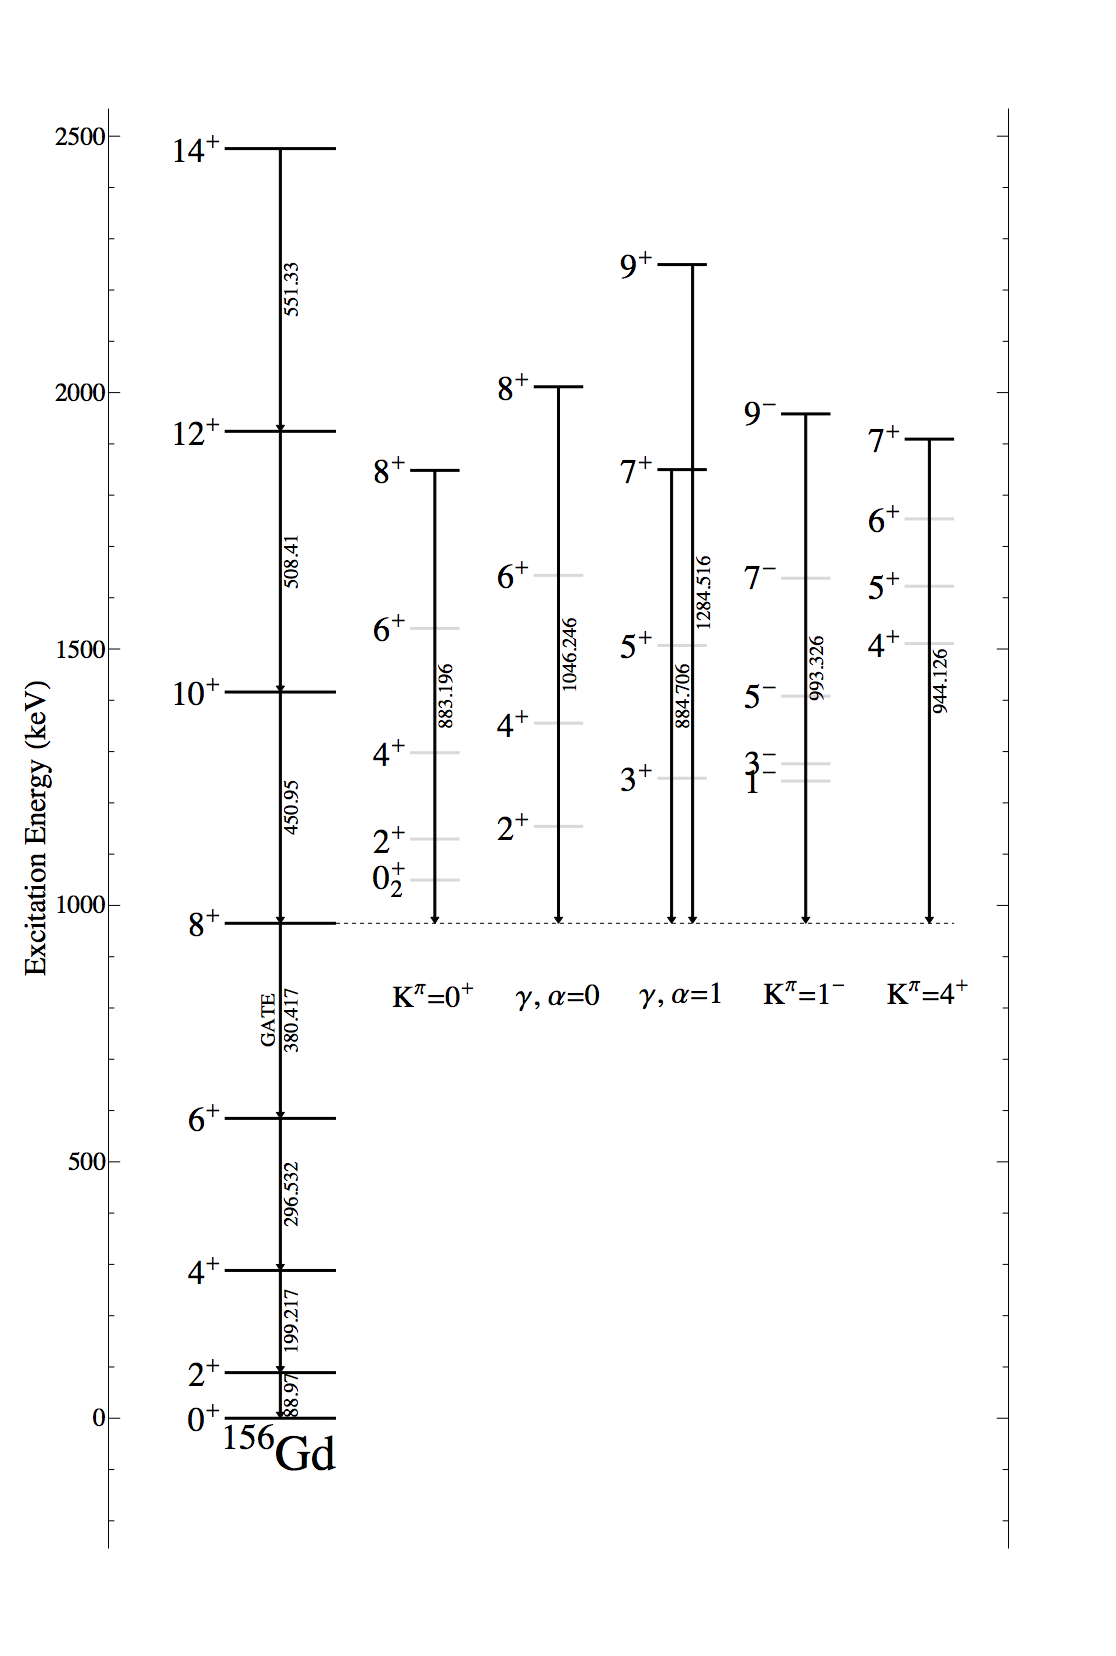
\includegraphics[scale=0.3]{156GdTablesAndFigs/156Gd_8to6.png}
    \caption{Level Scheme of $^{156}$Gd. The gamma ray of the $8^+$\rightarrow$6^+$ (380 keV) transition in the ground state was gated on. It was then compared with the gated spectrum from the gamma ray of the $10^+$\rightarrow$8^+$ (451 keV) transition in the ground state. Peaks only appearing in the first gate were assumed to go into the $8^+$ state, and assignments were made. Additionally, these peaks were also gated on, to look for cascades leading into the $8^+$ state, which were found in several cases. The levels are organized by band. The lower levels of the band, unseen by gamma rays in this gate, are in gray.}
    \label{fig:156_8to6}
\end{figure}}

Determining which transitions went uniquely into a given ground state level was done by comparing the outgoing ground state transition for that level with the incoming transitions, i.e. the $4^+\rightarrow2^+$ (199 keV) gate was compared directions with the $6^+\rightarrow4^+$ (296 keV) gate. The $\gamma$-spectra corresponding to these lines can be seen in Figure \ref{fig:156_GS_Gate}. Lines in the gamma spectrum that were present only in the outgoing spectrum, but not the incoming spectrum, are going into that level (the $4^+$ in the example above). Identified transitions were then gated on to confirm assignments and search for cascades from higher energy states.

\begin{figure}[!]
    \centering
    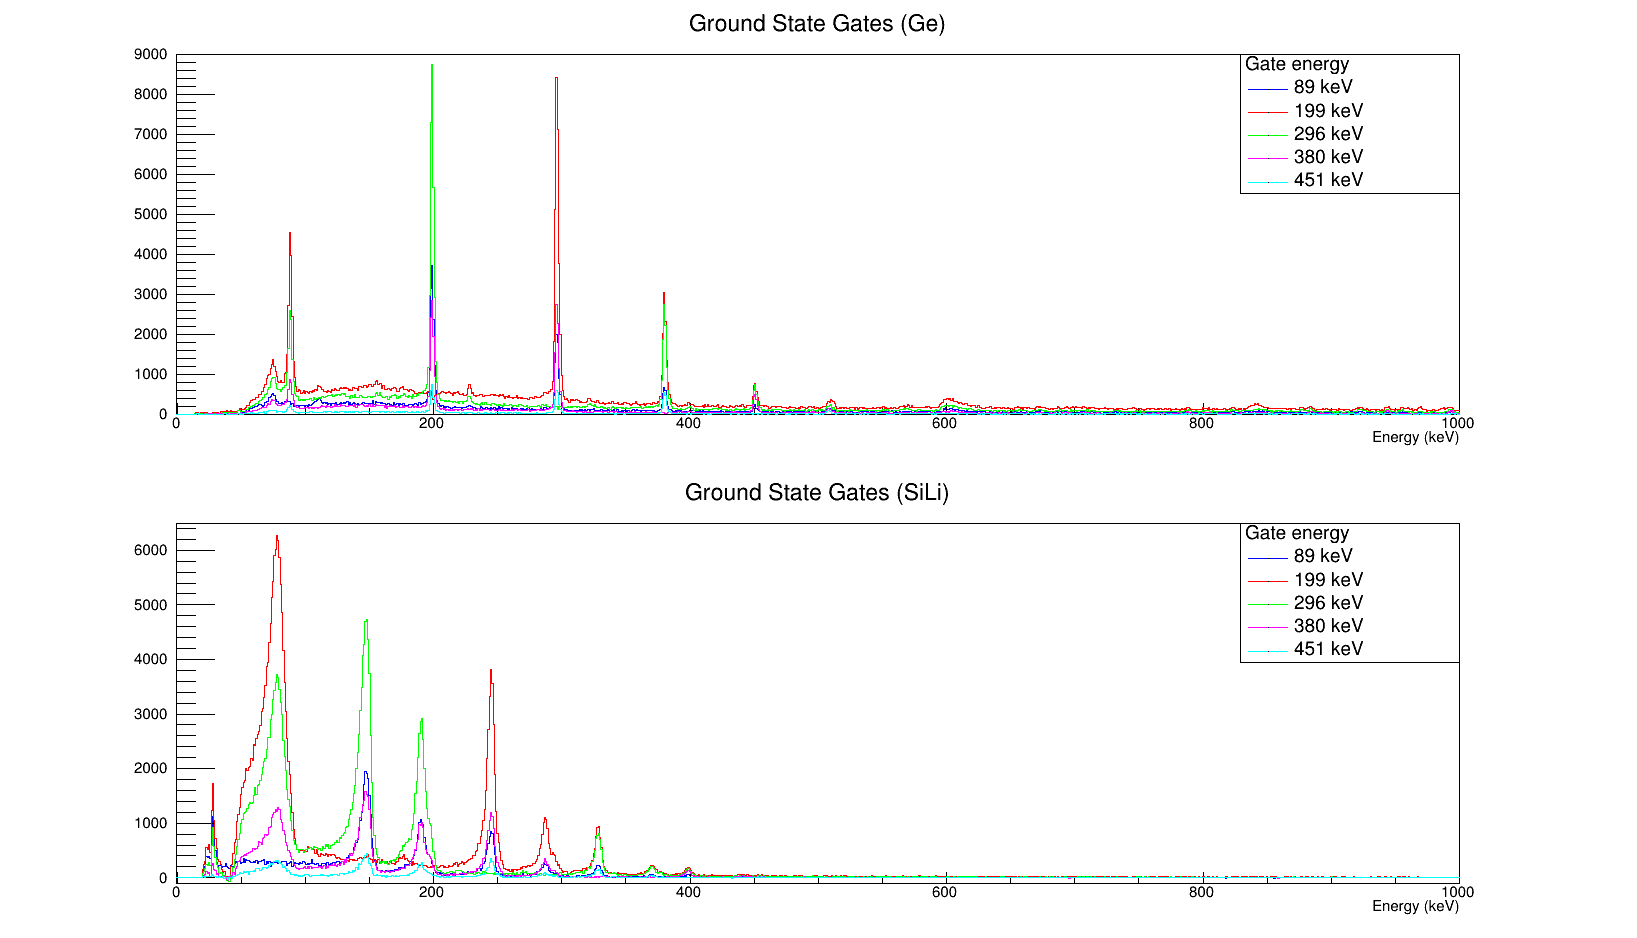
\includegraphics[scale=0.27]{156GdTablesAndFigs/156GS_stack.png}
    \caption{Spectra gated on the ground state band lines of $^{156}$Gd. As can be seen, some lines do not appear in different gates. Comparison of these gates, for instance 199 keV ($4^+\rightarrow2^+$) and 296 keV ($6^+\rightarrow4^+$), yields a list of transitions that directly populate the interim level (in the example, the $4^+$ state). The 89 keV line, although the lowest transition in the ground state band, has a low yield due to efficiency, and is reflected in the relative size of the peaks. The 199 keV peak in the gamma spectrum is much larger from the 296 keV transition than the 89 keV transition.}
    \label{fig:156_GS_Gate}
\end{figure}

In this data, the secondary gate check was especially important, as the low efficiency of the $2^+\rightarrow0^+$ transition would have meant weaker lines going into the $2^+$ state could be falsely assigned going into the $4^+$ state. As the ground state band transitions are so prolific, the transitions showed up when gating on weaker peaks in the spectra, while the inverse was not always true.

Little could be seen in the $2^+\rightarrow0^+$ gate, as it reflected in Figure \ref{fig:156_2to0}. The $4^+\rightarrow2^+$ gate shows far more, seen in Figure \ref{fig:156_4to2}, including evidence of populating 3 excited $0^+$ bands. In total, nine bands were seen in the gating outside of the ground state band. The number of bands seen drops off with higher gates, both due to the drop off in populating higher energy states and the drop off in populating higher $J$ states. Also seen in the gates are the $\gamma$-vibrational band, the $K=1^-$ octopole band, and a $K=4^+$ band.

\section{Conversion Coefficients from Singles}

With the gamma-rays now identified through gates, conversion coefficients could be calculated from singles spectra. Tables \ref{tab:156Gd_Single_ICC_Corr}, \ref{tab:156Gd_Single_ICC_Uncorr}, and \ref{tab:156Gd_No_Mult_ICC} are these results. Where available, results were compared with Konijn et al\citep{konijn81:_156gd}. Results are compared against this data, as it also examined the nucleus via an $(\alpha,2n)$ reaction.

Transitions that could be clearly identified and separated are found in Table \ref{tab:156Gd_Single_ICC_Corr}. Contamination concerns were taken into account by using the identified transitions to look for gamma-rays in close proximity to those in the Table. These transitions all have known multipole assignments and mixing ratios as needed, allowing for angular corrections. Two transitions with possible $E0$ components are seen in this Table. One, the $2^+\rightarrow2^+$ transition, appears to has a clear E0 component. Although this transition was not used in Figure \ref{fig:156_2to0}, the band the state exists in is populated, as seen in figures \ref{fig:156_4to2}, \ref{fig:156_6to4}, and \ref{fig:156_8to6}. The $6^+\rightarrow6^+$ transition does not appear to have an $E0$ component. While the value agrees with Konijn\citep{konijn81:_156gd}, it does not agree with the theoretical value for an $E2$, the multipole the transition has been assigned.

\afterpage{\clearpage\begin{landscape}
    \begin{longtable}{>{\footnotesize}c|>{\footnotesize}c|>{\footnotesize}c|>{\footnotesize}c|>{\footnotesize}c|>{\footnotesize}c|>{\footnotesize}c|>{\footnotesize}c|>{\footnotesize}c|>{\footnotesize}c|>{\footnotesize}c}
    \caption{$^{156}$Gd Internal Conversion Coefficients from Singles}
        \label{tab:156Gd_Single_ICC_Corr}\\
    \toprule
$E$ (keV)	&	$J^{\pi}	\rightarrow	J^{\pi}$	&	$E_i$ (keV)	&	$E_f$ (keV)	&	$T_{1/2}$ (fs)	&	Multipolarity	&	$\delta$	& Shell &	$\alpha$ (This Work)	&	$\alpha$  (Theory)\citep{kibedi08:_BRICC}	&	$\alpha$ (Konijn)\citep{konijn81:_156gd}	\\
\hline		
\endfirsthead
    \caption[]{$^{156}$Gd Internal Conversion Coefficients from Singles}\\
    \toprule
$E$ (keV)	&	$J^{\pi}	\rightarrow	J^{\pi}$	&	$E_i$ (keV)	&	$E_f$ (keV)	&	$T_{1/2}$ (fs)	&	Multipolarity	&	$\delta$ & Shell &	$\alpha$ (This Work)	&	$\alpha$  (Theory)\citep{kibedi08:_BRICC}	&	$\alpha$ (Konijn)\citep{konijn81:_156gd}	\\
\hline		
\endhead
\endfoot
\multicolumn{11}{p{1.4\textwidth}}{A list of conversion coefficients from $^{156}$Gd. Multipolarities and mixing ratios were taken from the nuclear date sheets\citep{reich12:_nds_156}. Unless otherwise stated, the $\alpha$ values are $\alpha_K$. An angular distribution correction has been applied based on multipolarities for pure transitions, and those with known mixing ratios. The first error is statistical, the second is systematic. Numbers are compared with Konijn et al\citep{konijn81:_156gd}.}
\endlastfoot
227.90	&	$7^-_{7^-}	\rightarrow 7^+_{4^+}$	&	2137.6	&	1909.26	&	1300000000	&	E1	&	& K	&	0.4687 (50)$^{+85}_{-84}$	&	0.0272 (4)	&	0.063 (13)	\\
	&			&		&		&		&		&	& LM	&	0.1073 (20) (20)	&	0.0049 (6)	&		\\ \hline
321.92	&	$8^-_{1^-}	\rightarrow	6^-_{1^-}$	&	2027.1	&	1705.799	&		&	E2	&		& K &	0.0290 (13) (9)	&	0.0378 (6)	&	0.025 (7)	\\ \hline
355.87	&	$4^+_{4^+}	\rightarrow	2^+_{\gamma}$	&	1510.594	&	1154.152	&	189000	&	E2	&		& K &	0.0158 (6) (5)	&	0.0281 (4)	&	\\ \hline
399.56	&	$9^+_{\gamma}	\rightarrow	7^+_{\gamma}$	&	2249.65	&	1849.84	&		&	E2	&		& K &	0.0077 (8) (3)	&	0.0205 (3)	&	0.026 (5)	\\ \hline
921.83	&	$5^+_{\gamma}	\rightarrow	6^+_{gs}$	&	1506.863	&	584.715	&	400	&	E2	&		& K &	0.0041 (9) (5) &	0.0028 (1)	&	0.0030 (7)	\\ \hline
1040.470	&	$2^+_{0^+_{2}}	\rightarrow	2^+_{gs}$	&	1129.437	&	88.970	&		&	E2+E0+M1	&	$-5.9^{+14}_{-28}$	& K &	0.0152 (10) (2)	&	0.0022 (1)	&	0.014 (3)	\\ \hline
1059.31	&	$6^+_{\gamma}	\rightarrow	6^+_{gs}$	&	1643.653	&	584.715	&		&	E2	&		& K &	0.0013 (5) (1)	&	0.0021 (1)	&	0.0013 (8)	\\ \bottomrule
    \end{longtable}
\end{landscape}}

Table \ref{tab:156Gd_Single_ICC_Uncorr} holds conversion coefficients that have been left uncorrected in the singles for one of two reaons: either there were multiple known assignments to the gamma-ray energy, or the exact multipole mixing-ratio $\delta$ was unknown. Several of these transitions are high energy $J^\pi\rightarrow J^\pi$ transitions if the assignment is correct without extra contamination. This includes a $0^+\rightarrow0^+$ transition. The Si(Li) efficiency at these energies was too low to see the conversion electrons in gated spectra.

\afterpage{\clearpage	\begin{ThreePartTable}
		\begin{longtable}{>{\footnotesize}c|>{\footnotesize}c|>{\footnotesize}c|>{\footnotesize}c|>{\footnotesize}c|>{\footnotesize}c|>{\footnotesize}c}
			\caption{Uncorrected $^{156}$Gd Internal Conversion Coefficients from Singles\label{tab:156Gd_Single_ICC_Uncorr} }\\
			\multicolumn{6}{c}{(a)} \\
			\toprule
	& & & & & \\
	$E$ (keV)	&	$J^{\pi}	\rightarrow	J^{\pi}$	&	$E_i$ (keV)	&	$E_f$ (keV)	& $T_{1/2}$ (fs) &	Multipolarity	&	$\delta$ \\
	\hline
	\endfirsthead
	\caption[]{Uncorrected $^{156}$Gd Internal Conversion Coefficients from Singles} \\
	\multicolumn{6}{c}{(a)} \\
	\toprule
	$E$ (keV)	&	$J^{\pi}	\rightarrow	J^{\pi}$	&	$E_i$ (keV)	&	$E_f$ (keV)	& $T_{1/2}$ (fs) &	Multipolarity	&	$\delta$ \\
	\hline
	\endhead
154.94	&	$4^+_{4^+}	\rightarrow	4^+_{\gamma}$	&	1510.594	&	1355.422	&	189000	&	M1+E2	&	0.48	\\
	&	$7^+_{4^+}	\rightarrow	6^+_{4^+}$	&	1909.26	&	1753.653	&		&	(M1+E2)	&	0.29	\\ \hline
883.86	&	$8^+_{0^+_{2}}	\rightarrow	8^+_{gs}$	&	1848.33	&	965.134	&		&	E0+E2	&		\\
	&	$7^+_{\gamma}	\rightarrow	8^+_{gs}$	&	1849.84	&	965.134	&		&	E2(+M1)	&		\\ 
	&		&		&	&		&	\\ \hline
955	&	$6^+_{0^+_{2}}	\rightarrow	6^+_{gs}$	&	1540.19	&	584.715	&		&	E0+E2	&		\\ 
959.88	&	$0^+_{0^+_{2}}	\rightarrow	2^+_{gs}$	&	1049.487	&	88.97	&	1800	&	E2	&			\\
	&	$3^+_{\gamma}	\rightarrow	4^+_{gs}$	&	1248.006	&	288.197	&	580	&	E2+M1	&	-12	\\ \hline
1009.33	&	$4^+_{0^+_{2}}	\rightarrow	4^+_{gs}$	&	1297.822	&	288.197	&	1600	&	E0+E2,M1	&		\\ 
&		&		&	&		&	\\ \hline
1045.48	&	$8^+_{\gamma}	\rightarrow	8^+_{gs}$	&	2011.38	&	965.134	&		&	E2(+M1)	&		\\ 
&		&		&	&		&	\\ 
1052.61	&	$7^-_{1^-}	\rightarrow	6^+_{gs}$	&	1638	&	584.715	&		&	E1	&		\\ \hline
1065.74	&	$2^+_{\gamma}	\rightarrow	2^+_{gs}$	&	1154.152	&	88.97	&	568	&	E2+M1	&	-16	\\
	&	$4^+_{\gamma}	\rightarrow	4^+_{gs}$	&	1355.422	&	288.187	&	540	&	E2+M1	&	-4	\\ \hline
1158.65	&	$2^+_{\gamma}	\rightarrow	0^+_{gs}$	&	1154.152	&	0	&	568	&	E2	&		\\
	&	$3^+_{\gamma}	\rightarrow	2^+_{gs}$	&	1248.006	&	88.97	&	580	&	E2+M1	&	-11.8	\\ \hline
1168.69	&	$0^+_{0^+_{3}}	\rightarrow	0^+_{gs}$	&	1168.186	&	0	&	5000	&	E0	&		\\
	&	$2^+_{0^+_{3}}	\rightarrow	2^+_{gs}$	&	1258.075	&	88.97	&	1540	&	E2+M1+E0	&	0.38	\\ \hline
1222.22	&	$4^+_{4^+}	\rightarrow	4^+_{gs}$	&	1510.594	&	288.197	&	189000	&	M1+E2	&	-1.7	\\
	&	$5^+_{\gamma}	\rightarrow	4^+_{gs}$	&	1506.863	&	288.197	&	400	&	E2	&		\\ \hline
1264.85	&	$4^+_{\gamma}	\rightarrow	2^+_{gs}$	&	1355.422	&	88.97	&	540	&	E2	&		\\
	&	$8^+_2	\rightarrow	6^+_{gs}$	&	1848.33	&	584.715	&		&		\\
	&	$7^+_{\gamma}	\rightarrow	6^+_{gs}$	&	1849.84	&	584.715	&		&		\\ 
	&		&		&	&		&	\\ 
	\bottomrule
\end{longtable}
\end{ThreePartTable}
\pagebreak
\begin{ThreePartTable}
	\begin{TableNotes}[para]
		Table \ref{tab:156Gd_Single_ICC_Uncorr}: A list of conversion coefficients from $^{156}$Gd. Multipolarities and mixing ratios were taken from the nuclear data sheets\citep{reich12:_nds_156}. Unless otherwise stated, the $\alpha$ values are $\alpha_K$. No angular distribution correction has been applied, either due to unknown mixing ratios, or multiple assignments of the gamma-ray. The first error is statistical, the second is systematic. Numbers are compared with Konijn et al. \citep{konijn81:_156gd} Starred values were used as calibration points in the Konijn paper. All coefficients are K-shell electrons.
	 \end{TableNotes}
\begin{longtable*}{>{\footnotesize}c|>{\footnotesize}c|>{\footnotesize}c|>{\footnotesize}c|>{\footnotesize}c|>{\footnotesize}c}
	%\multicolumn{6}{c}{\MakeUppercase{Table \ref{tab:156Gd_Single_ICC_Uncorr} (Continued)}} \\
	\multicolumn{6}{c}{\MakeUppercase{Table 5.4 (Continued)}} \\
	\multicolumn{6}{c}{(b)} \\
	\toprule
	&  & \multicolumn{2}{>{\footnotesize}c|}{$\alpha$ (This Work)} & & \\
	$E$ (keV)	& Shell	&	Uncorrected & Corrected &	$\alpha$  (Th)\citep{kibedi08:_BRICC}	&	$\alpha$ (Konijn)\citep{konijn81:_156gd} \\
	\hline
	\endfirsthead
	%\multicolumn{6}{c}{\MakeUppercase{Table \ref{tab:156Gd_Single_ICC_Uncorr} (Continued)}} \\
	\multicolumn{6}{c}{\MakeUppercase{Table 5.4 (Continued)}} \\
	\multicolumn{6}{c}{(b)} \\
	\toprule
	&  & \multicolumn{2}{>{\footnotesize}c|}{$\alpha$ (This Work)} & & \\
	$E$ (keV)	& Shell	&	Uncorrected & Corrected &	$\alpha$  (Th)\citep{kibedi08:_BRICC}	&	$\alpha$ (Konijn)\citep{konijn81:_156gd} \\
	\hline
	\endhead
	154.94	& K & 	0.4635 (183)$^{+98}_{-97}$	& 0.3462 (137)$^{+73}_{-72}$ &	0.460 (7)	& \\
	&		 K &	0.4879 (193)$^{+103}_{-102}$ &	0.474 (7)	&		\\ \hline
883.86	& K &	0.0057 (7) (1)	& 0.0034 (4) (1) &	0.0030 (1)	& $>0.0092$		\\
& K &		&	[M1] 0.0102 (13) (2) & [M1] 0.0052 (1)	&	$<0.0052$	\\ 
&  &		&	[E2] 0.0073 (9) (1) & [E2] 0.0030 (1)	&		\\ \hline
955	& K &	0.0065 (4) (5)	& 0.0039 (2) (3) &	0.0026 (1)	&	0.020 (8)	\\ 
959.88	& K & &	0.0136 (8) (10) &  0.0025 (1)	&	0.0045 (24)	\\
& K &		&	0.0120 (7) (9) & 0.0025 (1)	&		\\ \hline
1009.33	& K &	0.0173 (9) (4)	& [M1] 0.0234 (12) (5) &	[M1] 0.0038 (1)	&	0.0164 (29)	\\ 
&  &		&	[E2] 0.0107 (6) (2) & [E2] 0.0023 (1)	&		\\ \hline
1045.48	& K &	0.0012 (2) (2)	& [M1] 0.0015 (3) (3)	 & [M1] 0.0035 (1)	&	0.0025 (6)	\\ 
&  &		&	[E2] 0.0007 (1) (1) & [E2] 0.0021 (1)	&		\\ 
1052.61	& K & &  0.0008 (1) (1)	&	0.0009 (1)	&		\\ \hline
1065.74	& K &	0.0023 (2) (1)	& 0.0034 (3) (1) &	0.0021 (1)	&	0.0025 (9)	\\
& K &		&	0.0029 (3) (1) & 0.0021 (3)	&	0.0021 (1)	\\ \hline
1158.65	& K &	0.0020 (3) (1)	& 0.0020 (3) (1) &	0.0017 (1)	&	0.0023 (3)	\\
& K & & 0.0014 (2) (1)		&	0.0017 (1)	&		\\ \hline
1168.69	& K &	0.0045 (3) (1)	& 0.0045 (3) (1) & 		&	$>0.0035$	\\
& K &	& 0.0038 (3) (1)	&	0.0026 (1)	&		\\ \hline
1222.22	& K &	0.0028 (4) (1)	 & 0.0031 (4) (1) &	0.0018 (1)	&	0.00174*	\\
& K &		& 0.0031 (4) (1)	& 0.001560 (22)	&	\\ \hline
1264.85	& K &	0.0017 (3) (1) & 0.0014 (2) (1)	&	0.0014 (1)	&	\\
& K &		& [E2] 0.0014 (2) (1)	&	[E2] 0.0014 (1) &		\\
& K &		& [M1] 0.0011 (2) (1)	& [M1] 0.0022 (1)	&		\\ 
&		&		&	[E2] 0.020 (3) (1) & [E2] 0.0014 (1)	&		\\
	\bottomrule
	\insertTableNotes
\end{longtable*}

\end{ThreePartTable}}

Table \ref{tab:156Gd_No_Mult_ICC} has conversion coefficients that could not be corrected due to the transitions having unknown multipole assignments. Allowable and reasonable theoretical conversion coefficients from BrIcc\citep{kibedi08:_BRICC} are listed in the table.

\afterpage{\clearpage\begin{landscape}
    \begin{longtable}{c|c|c|c|c|c|c|c|c}
        \caption{$^{156}$Gd Internal Conversion Electrons without known Multipolarities}
        \label{tab:156Gd_No_Mult_ICC}\\
        \toprule
        &	& 	&  &	& \multicolumn{2}{c}{Theory}	& 	\\
        $E_i$ (keV)	&	$E_f$ (keV)	& $E$ (keV)	&	Gate &		$\alpha$ (This Work)	& $\alpha$(M1) & $\alpha$(E2) & $\alpha$(E1) &	$\alpha$ (Konijn)	\\
        \hline		
        \endfirsthead
        \caption[]{$^{156}$Gd Internal Conversion Electrons without known Multipolarities}\\
        \toprule
        &	& 	&  &	& \multicolumn{2}{c}{Theory}	& 	\\
        $E_i$ (keV)	&	$E_f$ (keV)	& $E$ (keV)	&	Gate &		$\alpha$ (This Work)	& $\alpha$(M1) & $\alpha$(E2) & $\alpha$(E1) &	$\alpha$ (Konijn)	\\
        \hline		
        \endhead
        671.41	&	$7^-	\rightarrow	8^+$	&	1638	&	965.134	&		0.0064 (6) (2)	& & & 0.00213 (3) &	\\ \hline
        838.83	&	$9^+	\rightarrow	10^+$	&	2249.65	&	1416.078	&	0.0009 (3) (1)	& 0.00595 (9) & 0.00337 (5) & & 	\\ \hline
        943.732	&	$7^+	\rightarrow	8^+$	&	1909.26	&	965.134		&	0.0022 (6) (1) & 0.00448 (7) & 0.00262 (4) & &	0.0025 (3)	\\ 
        \bottomrule
    \end{longtable}
    \caption{A list of conversion coefficients from $^{156}$Gd without known multipolarities. As a result, an angular distribution correction term has not been applied. None of the states have known half lives. The first error is statistical, the second is systematic. Numbers are compared with theoretical values for allowed multipolarities and results from Konijn et al. \citep{konjin81:_156gd}. All coefficients are K-shell electrons.}
\end{landscape}}

\section{$J^{\pi}\rightarrow J^{\pi}$ Transitions}

After identification of the bands and transitions, gates were put on the transitions both entering and leaving states of interest, namely even-$J^+$ states. Gates entering these states (incoming transitions) were not fruitful. This is unfortunate for the $0^+$ states, as only incoming transitions can be used for transitions to the ground state. Gates leaving the states (outgoing transitions), had more statistics, and results could be obtained. $J^\pi\rightarrow J^\pi$ transitions up to $4^+$ were seen. Tables \ref{tab:156Gd_0_to_0}, \ref{tab:156Gd_2_to_2}, and \ref{tab:156Gd_4_to_4} are the tabulated results. These values are compared with Konijn\citep{konijn81:_156gd} where available. Additionally, the theoretical conversion coefficients have been listed for the $M1$ and $E2$ transitions, as taken from BrIcc\citep{kibedi08:_BRICC}.

In Table \ref{tab:156Gd_0_to_0}, only one $0^+\rightarrow0^+$ transition could be seen with enough statistics to get a value. All other possible $0^+\rightarrow0^+$ transitions were at high energies with such low efficiency in the Si(Li) detectors that a peak could not be seen.
    
\afterpage{\clearpage\begin{landscape}
    \begin{longtable}{c|c|c|c|c|c|c|c|c}
        \caption{$0^+\rightarrow 0^+$ Transitions in $^{156}$Gd}
        \label{tab:156Gd_0_to_0}\\
        \toprule
        &	& & & 	&  &	& \multicolumn{2}{c}{Theory}	\\
        $E_i$ (keV)	& Band &	$E_f$ (keV)	& Band &$E$ (keV)	&	Gate &		$\alpha$ (This Work)	& $\alpha$(M1) & $\alpha$(E2) \\
        \hline
        \endfirsthead
        \toprule
        \caption[]{$0^+\rightarrow 0^+$ Transitions in $^{156}$Gd}\\
        & & &	& 	&  &	& \multicolumn{2}{c}{Theory}	\\
        $E_i$ (keV)	& Band &	$E_f$ (keV)	& Band &$E$ (keV)	&	Gate &		$\alpha$ (This Work)	& $\alpha$(M1) & $\alpha$(E2) \\
	    \endhead
	    \endfoot
	    \multicolumn{9}{p{1.4\textwidth}}{A list of conversion coefficients from $^{156}$Gd for $0^+\rightarrow 0^+$ transitions seen in the gated data. All listed theoretical values are for the K-shell internal conversion coefficient. Numbers are compared with theoretical values for illustration. All coefficients are K-shell electrons. }
	    \endlastfoot
        1168.186 & $0^+_{3}$ & 1049.487  & $0^+_{2}$ & 118.71 &  960.50771 & $>1.1970$ & 1.042 (15) & 0.726 (11) \\
        \bottomrule
    \end{longtable}
\end{landscape}}

In Table \ref{tab:156Gd_2_to_2}, only one transition had a previously measured value. It does not appear to have an $E0$ component. The other transitions with upper limits do not eliminate the possibility of an $E0$ component. Of the two transitions with lower limits, one (104 keV) appears to have a sizeable $E0$ component, while the other transition does not eliminate the possibility of a pure $E2$ transition.

\afterpage{\clearpage\begin{landscape}
    \begin{longtable}{c|c|c|c|c|c|c|c|c|c}
        \caption{$2^+\rightarrow 2^+$ Transitions in $^{156}$Gd}
        \label{tab:156Gd_2_to_2}\\
        \toprule
        & & &	& 	&  &	& \multicolumn{2}{c|}{Theory\citep{kibedi08:_BRICC}}	& 	\\
        $E_i$ (keV)	& Band &	$E_f$ (keV)	& Band &$E$ (keV)	&	Gate &		$\alpha$ (This Work)	& $\alpha$(M1) & $\alpha$(E2) &	$\alpha$ (Konijn)	\\
        \hline
        \endfirsthead
        \toprule
        \caption[]{$2^+\rightarrow 2^+$ Transitions in $^{156}$Gd}\\
        & & &	& 	&  &	& \multicolumn{2}{c|}{Theory\citep{kibedi08:_BRICC}}	& 	\\
        $E_i$ (keV)	& Band &	$E_f$ (keV)	& Band &$E$ (keV)	&	Gate &		$\alpha$ (This Work)	& $\alpha$(M1) & $\alpha$(E2) &	$\alpha$ (Konijn)	\\
        \hline
	    \endhead
	    \endfoot
	    \multicolumn{10}{p{1.4\textwidth}}{A list of conversion coefficients from $^{156}$Gd for $2^+\rightarrow 2^+$ transitions seen in the gated data. All listed theoretical values are for the K-shell internal conversion coefficient. Numbers are compared with Konijn et al.\citep{konijn81:_156gd} All coefficients are K-shell electrons. }
	    \endlastfoot
        1258.075 & $0^+_{3}$ & 1129.437 & $0^+_{2}$ & 128.638 & 1040.470 & $>0.5325$ & 0.830 (12) & 0.578 (8) &\\ \hline
        1258.075 & $0^+_{3}$ & 1154.152 & $\gamma$ & 103.92 & 1065.1781 & $>2.9695$ & 1.524 (22)  & 1.049 (15) &\\ \hline
        1827.841 & $2^+_2$ & 1129.437 & $0^+_{2}$ & 698.407 & 1040.470 & $<0.0208$ & 0.00932 (13) & 0.00506 (7) & \\ \hline
        1827.841 & $2^+_2$ & 1154.152 & $\gamma$ & 673.684 & 1065.1781 & $<0.0228$ & 0.01018 (15) & 0.00550 (8) &\\ \hline
        1827.841 & $2^+_2$ & 1258.075 & $0^+_{3}$ & 569.771 & 1169.087 & $<0.0013$ & 0.01545 (22) & 0.00819 (12) & 0.006 (4) \\
        \bottomrule
    \end{longtable}
\end{landscape}}
   
In Table \ref{tab:156Gd_4_to_4}, none of the transitions had a previously measured value. Three of the four transitions' lower limits give no new information. The final one appears to indicate there is an $E0$ component, with the lower limit higher than the theoretical $M1$ coefficient. 
   
\afterpage{\clearpage\begin{landscape}
    \begin{longtable}{c|c|c|c|c|c|c|c}
        \caption{$4^+\rightarrow 4^+$ Transitions in $^{156}$Gd}
        \label{tab:156Gd_4_to_4}\\
        \toprule
        &	& 	&  &	& \multicolumn{2}{c}{Theory}	& 	\\
        $E_i$ (keV)	&	$E_f$ (keV)	& $E$ (keV)	&	Gate &		$\alpha$ (This Work)	& $\alpha$(M1) & $\alpha$(E2) &	$\alpha$ (Konijn)	\\
        \hline
        \endfirsthead
        \toprule
        \caption[]{$4^+\rightarrow 4^+$ Transitions in $^{156}$Gd}\\
        &	& 	&  &	& \multicolumn{2}{c}{Theory}	& 	\\
        $E_i$ (keV)	&	$E_f$ (keV)	& $E$ (keV)	&	Gate &		$\alpha$ (This Work)	& $\alpha$(M1) & $\alpha$(E2) &	$\alpha$ (Konijn)	\\
        \hline
	    \endhead
        1462.297 & 1297.822 & 164.469 & 1009.649 & $>0.4870$ & 0.416 (6) & 0.279 (4) & \\ \hline
        1462.297 & 1355.422 & 106.88 & 1067.2325 & $>0.7233$ & 1.405 (20) & 0.972 (14) & \\ \hline
        1510.594 & 1297.822 & 212.771 & 1009.649 & $>0.0704$  & 0.204 (3) & 0.1282 (18) & \\ \hline
        1510.594 & 1355.422 & 155.168 & 1067.2325 & $>0.0981$ & 0.490 (7) & 0.333 (5) &  \\
        \bottomrule
    \end{longtable}
    \caption{A list of conversion coefficients from $^{156}$Gd for $4^+\rightarrow 4^+$ transitions seen in the gated data. All listed theoretical values are for the K-shell internal conversion coefficient. Numbers are compared with Konijn et al. \citep{konjin81:_156gd} All coefficients are K-shell electrons.}
\end{landscape} }

Due to the lack of lifetimes of these states, $B(E0)$ values cannot be calculated. However, the relative intensities of these values can be compared, assuming they are coming from the same state, as the lifetime would divide out (see equation \ref{eq:BEO}). The contributions from the individual components of the transition must be separated out for the $2^+$ and $4^+$ transitions. This was done by getting the $q^2$ values multiplied by the theoretical $\alpha(E2)$, which gives an estimate of $E0$ intensity, sans a normalization (see equation \ref{eq:mixedE0}). None of the transitions have known $\delta$ mixing ratios, so $\delta$ was assumed to be 1, and the theoretical mixed $M1$ and $E2$ $\alpha$ was subtracted. In some cases, this left a negative value, which has been excluded from the table of results, Table \ref{tab:156Gd_E0}. All values calculated are upper or lower limits, as the $\alpha$ calculated in the previous tables were upper and lower limits.

\afterpage{\clearpage\begin{portrait}
    \begin{longtable}{c|c|c|c|c}
        \caption{$E0$ Contributions for $J^{\pi}\rightarrow J^{\pi}$ Transitions}
        \label{tab:156Gd_E0}\\
        \toprule
        $E_i$ (keV)	&	$E_f$ (keV)	& $E$ (keV)	&	Gate &		$q^2\alpha(E2)$		\\
        \hline
        \endfirsthead
        \toprule
        \caption{$E0$ Contributions for $J^{\pi}\rightarrow J^{\pi}$ Transitions} \\
        $E_i$ (keV)	&	$E_f$ (keV)	& $E$ (keV)	&	Gate &		$q^2\alpha(E2)$		\\
        \hline
	    \endhead
	    \multicolumn{5}{l}{$0^+\rightarrow 0^+$} 	\\ \hline
        1168.186 & 1049.187 &  118.71 & 960.50771 & $>0.626$ \\\hline
        \multicolumn{5}{l}{$2^+\rightarrow 2^+$} 	\\ \hline
        1258.075 & 1154.152 & 103.92 & 1065.1781 & $>3.366$  \\ \hline
        1827.841 & 1129.437 & 698.407 & 1040.47 & $<0.02722$  \\ \hline
        1827.841 & 1154.152 & 673.684 & 1065.1781 & $<0.02992$  \\ \hline
        \multicolumn{5}{l}{$4^+\rightarrow 4^+$} 	\\ \hline
        1462.297 & 1297.822 & 164.469 & 1009.649 &  $>0.279$  \\
        \bottomrule
	\end{longtable}
    \item{A list of E0 contributions in $^{156}Gd$. These values have not been normalized, as the lifetime of the states are unknown. The $0^+\rightarrow 0^+$ transitions list the $\alpha(expt)$, as $M1$ and $E2$ transitions are forbidden. Table \ref{tab:156Gd_BE0_Comp} compares values between two transitions of the same initial state. Only non-negative values are listed in the table, and $\delta$ was assumed to be 1, as no mixing ratios are known for these transitions. For $\alpha(exp)$, $\alpha(M1)$, and $\alpha(E2)$ used in these calculations, please refer to Tables \ref{tab:156Gd_0_to_0}-\ref{tab:156Gd_4_to_4}.}
\end{portrait}}

With these values, two transitions from the same level can be compared using the $B(E0)$ formula to take the energy adjustment into account. It is also adjusted by the ratio of the rate efficiencies. Only one $2^+$ level had transitions to other $2^+$ states that could be compared. This ratio is in Table \ref{tab:156Gd_BE0_Comp}. There is no error, as the two compared values were both upper limits. The number seems to indicate the 1827 keV level has approximately equal transition strength to the 1129 keV and the 1154 keV $2^+$ states.

\afterpage{\clearpage
    \begin{longtable}{c|c|c|c|c|c|c}
        \caption{$B(E0)$ Ratios for $J^{\pi}\rightarrow J^{\pi}$ Transitions}
        \label{tab:156Gd_BE0_Comp}\\
        \toprule
        $E_i$ (keV)	& Band &	$E_{0^+_2}$ (keV)	& Gate$_{0^+_2}$ & $E_{\gamma}$ (keV)	& Gate$_{\gamma}$ &	$B(E0)$	Ratio	\\
        \hline
        \endfirsthead
        \toprule
        \caption{$B(E0)$ Ratios for $J^{\pi}\rightarrow J^{\pi}$ Transitions} \\
        $E_i$ (keV)	& Band &	$E_{0^+_2}$ (keV)	& Gate$_{0^+_2}$ & $E_{\gamma}$ (keV)	& Gate$_{\gamma}$ &	$B(E0)$	Ratio	\\
        \hline
	    \endhead
	    \endfoot
	    \multicolumn{7}{p{\textwidth}}{Ratios of the $B(E0)$ values in $^{156}$Gd. Only ratios between two transitions of the same state are listed, as the lifetime of the states are unknown. Table \ref{tab:156Gd_E0} lists the values that were used in the calculation. The gates are included, as an efficiency correction was made on the ratio based on the gates. In many cases, only upper or lower limits for the values could be used for this calculation. Errors are not given on these values.}
	    \endlastfoot
        \multicolumn{6}{l}{$2^+\rightarrow 2^+$} 	\\ \hline
        1827.841 & $2^+_2$ & 1129.437 & 1040.47 & 1154.152 & 1065.1781 & 1.128  \\
        \bottomrule
	\end{longtable}
}